\documentclass[12pt]{article}

% PACKAGES
\usepackage[ngerman]{babel}
\usepackage{lmodern} % Schriftart
\usepackage{bookmark} % Für PDF Lesezeichen
\usepackage{caption} % Für \caption*{}
\usepackage{siunitx} % SI-Einheiten
\usepackage{mathtools} % Verbessertes "amsmath" (https://de.overleaf.com/learn/latex/Articles%2FMathtools_-_for_beautiful_math)
\usepackage{xcolor}   % Farbiger Text (https://www.overleaf.com/learn/latex/Using_colours_in_LaTeX)
\usepackage{geometry} % Zur Einstellung des Layouts
\usepackage{titlesec} % Einteilung des Inhalts (https://de.overleaf.com/learn/latex/Sections_and_chapters)
\usepackage{fancyhdr} % Für Kopf-/ und Fußzeilen (https://www.overleaf.com/learn/latex/Headers_and_footers)
\usepackage{parskip} % Änderung von Absätzen und Absatzeinzügen
\usepackage{biblatex} % Verweise und Referenzen
\usepackage{float} % Benötogt für Figuren und Tabellen
\usepackage{graphicx} % Platzhalter Bilder
\usepackage{booktabs} % Tabellen
\usepackage{csquotes} % Recommended package for biblatex
\usepackage{hyphenat}
% SETUP 
\setlength{\headheight}{15.059pt} % Set headheight to at least 14.5pt
\addtolength{\topmargin}{-2.5pt} % Make topmargin smaller to compensate
\sisetup{
  per-mode=fraction,
  fraction-function=\tfrac,
  separate-uncertainty=true
}
\addbibresource{Ressourcen/V44.bib}
\geometry{ %A4
  a4paper,
  total = {170mm,240mm},
  left = 20mm,
  top = 30mm
}
\pagestyle{fancy}
\captionsetup[figure]{
    justification=centering, % Centered captions
    labelsep=colon, % Separate label and caption with a period
    singlelinecheck=false, % Always center even if the caption is short
    labelfont=bf % Bold captions
}
% COMMANDS
\newcommand{\uproman}[1]{\uppercase\expandafter{\romannumeral#1}} % Römische Zahlen


% DOC
\begin{document}

% HEADER
\begin{titlepage}
  \centering
  \vspace*{1cm}
  
\includegraphics[width=0.5\textwidth]{Ressourcen/tud_logo_schwarz(RGB)}\\
  \vspace*{0.25cm}
  \large\textmd{Fakultät Physik} \\
  \vspace*{6cm}
  \huge \bfseries FP-2024 - Versuch V44\\
  \vspace*{0.25cm}
  \large Röntgenreflektometrie\\
  \vspace*{0.25cm}
  \large\textmd{\href{mailto:martin.boussard@tu-dortmund.de}{Martin Boussard}} \\
  \large\textmd{\href{mailto:jan.oppoli@tu-dortmund.de}{Jan Oppoli}} \\
  \vfill
  \small\textmd{Versuch durchgeführt am 22. April 2024}\\
  \small\textmd{Abgabe erstellt am \today}
\end{titlepage}
\tableofcontents 
\newpage

\section{Zielsetzung}\label{sec:zielsetzung}
Ziel dieses Versuchs ist es, verschiedene physikalische bzw. geometrische Eigenschaften wie Elektronendichte, Schichtdicke oder Rauigkeit eines Polysterolfilms auf einem Siliziumwafer mittels der Röntgen-reflektometrie zu bestimmen.
Die Untersuchung/ Kontrolle solcher Schichten im Nanometerbereich ist insbesondere innerhalb der Halbleiterelektronik von Bedeutung und besitzt eine hohe Relevanz für die Industrie.
Durch Analyse des Resultierenden Streubildes unter Verwendung problemangepasster Algorithmen können charakteristische Strukturinformationen der Probe gewonnen werden.
\section{Theorie}\label{sec:theorie}
Als Grundlage für eine effiziente Auswertung der Daten müssen zunächst einige wichtige physikalische Phänomene bzw. Modelle erläutert werden.
\subsection{Röntgenstrahlung}\label{subsec:röntgen}
Aufgrund ihrer relativ zum sichtbaren Licht vergleichsweise kleine Wellenlänge 
\begin{align*}
  \lambda_{\text{Röntgen}} < \SI{10}{\nano\meter} < \SI{400}{\nano\meter} <\lambda_\text{Sichtbar}
\end{align*}
eignet sich Röntgenstrahlung ideal zur Untersuchung von Strukturen der selben Größenordnung.
\subsubsection{Erzeugung von Röntgenstrahlung}
Nachdem mithilfe des Glühelektrischen Effekts aus der Kathode herausgelöste Elektronen innerhalb der Röntgenröhre in Richtung der Anode beschleunigt werden, wird bei dem Auftreffen Röntgenstrahlung erzeugt.
Hierbei ist zwischen Bremsstrahlung und dem charakteristischen Röntgenspektrum zu unterscheiden, wie in \autoref{fig:1} veranschaulicht ist.
\begin{itemize}
  \item \textbf{Bremsstrahlung}:\\Die durch Coulombwechselwirkung zwischen Elektron und Atomrumpf des Targets verkleinerte kinetische Energie des Elektrons wird teilweise in Röntgenstrahlung mit kontinuierlichem Spektrum umgewandelt und emittiert.
  \item \textbf{Charakteristische Röntgenstrahlung}:\\Treffen die beschleunigten Elektronen auf das Target und lösen dort Elektronen aus inneren Schalen des Atoms heraus, werden diese Leerstellen durch nachrückende Elektronen aus höheren Schalen gefüllt und die resultierende Energiedifferenz spiegelt sich in der Emission von Röntgenstrahlung diskreter Frequenzen wieder, da die Übergangsenergien im Atom quantisiert sind.
\end{itemize}
\begin{figure}[H]
  \centering
  \includegraphics[scale=0.5]{Ressourcen/Röntgenspektrum.png}
  \caption{Schematisches Emissionsspektrum einer Kupferanode, wie auch\\in diesem Versuch verwendet.\cite{ROEDresden}}\label{fig:1}
\end{figure}
\subsubsection{Eigenschaften von Röntgenstrahlung}
Die in diesem Versuch relevanteste Frequenz ist die sog. $\text{K}_\alpha$-Linie, welche einem Übergang eines Elektrons von der zweiten(M) in die erste(K) Schale und der Wellenlänge $\lambda_{\text{K}_\alpha}=\SI{0.1514}{\nano\meter}$ entspricht\cite{ekabs}.
Die zugehörige Frequenz $\omega$ liegt weit über jeglichen Resonanzfrequenzen $\omega_1$ der betrachteten Materialien, was für weitere theoretische Betrachtungen von Bedeutung ist.
\subsubsection{Röntgenstrahlung an Grenzflächen}
Das Verhalten von Röntgenstrahlung an Grenzflächen von Medien unterschiedlichem Brechungsindexes wird gemäß des Snelluis'schen Brechungsgesetzes
\begin{align}
  n_1 \cos(\alpha) = n_2 \cos(\alpha_\text{t})\label{eq:snellius}
\end{align}
entsprechend der Winkel in \autoref{fig:2} dargestellt, wobei nach dem Reflexionsgesetz Einfallswinkel = Ausfallswinkel gilt.
\begin{figure}[H]
  \centering
  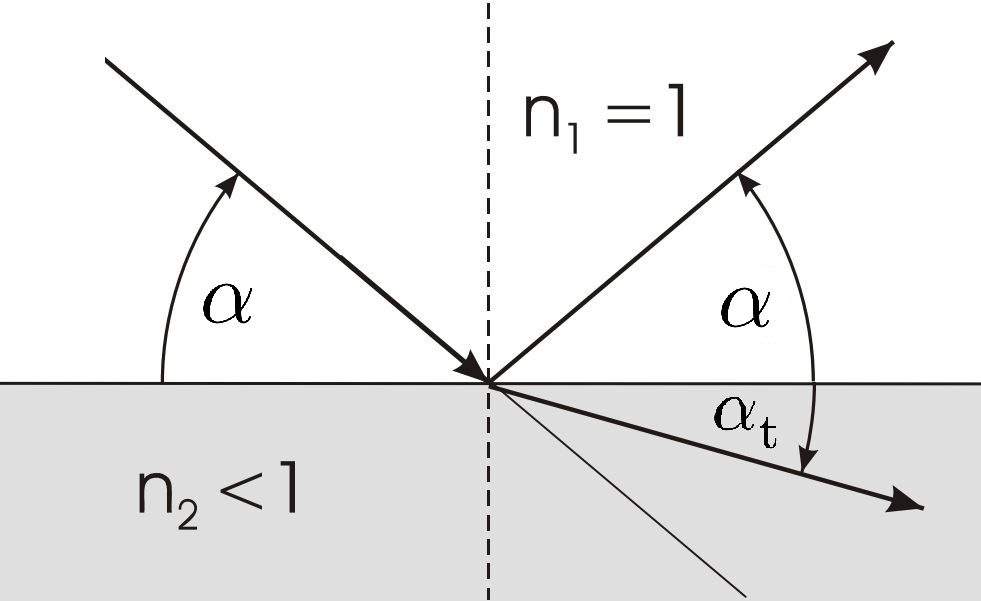
\includegraphics[scale=0.3]{Ressourcen/Snellius.png}
  \caption{Skizze der Winkel des einfallenden, ausfallenden und\\ gebrochenen Strahls and einer Grenzfläche.}\cite{uni_giessen}\label{fig:2}
\end{figure}
Der komplexe Brechungsindex $n$ von verschiedenen Medien, welcher die variierte Lichtgeschwindigkeit im jeweiligen Material beschreibt, rührt von Lorentz-Oszillator-Modell für Fest-körper her, bei welchem sich im hochfrequenten Näherungsfall der Röntgenstrahlung die folgende Formel für nicht-ferromagnetische Materialien  
\begin{align}
  n=\sqrt{\epsilon_\text{r}}=1-\frac{\rho r_0}{2\pi}\lambda^2+i \frac{\gamma}{4\pi}\lambda \coloneqq 1-\delta+i\beta\label{eq:n}
\end{align}
mit Elektronenradius $r_0$, Elektronendichte $\rho$, Wellenlänge $\lambda$ und linearem Absorptionskoeffizient $\gamma$ zusammengefasst in Kenngrößen der Dispersion $\delta$ und der Absorption $\beta$, ergibt. 
\\\linebreak Besonderheit der Röntgenstrahlung ist, dass für sie jedes Medium geringfügig optisch dünner als das Vakuum erscheint, womit im Gegensatz zu sichtbarem Licht Totalreflexion im Übergang von Vakuum zu Medium auftreten kann.
Dies tritt gemäß \autoref{eq:snellius}, \ref{eq:n} für Winkel kleiner als
\begin{align}
  \alpha_\text{Krit} = \sqrt{2 \delta} = \lambda \sqrt{\frac{\rho r_0}{\pi}}\label{eqn:a_krit}
\end{align}
auf, da der Cosinus für derart kleine betrachtete Winkel mithilfe seiner Taylorreihe angenährt werden kann.
Somit gilt die Formel
\begin{align}
  \alpha_\text{t} = \sqrt{\alpha^2-2\delta}\text{.}
\end{align}
\subsection{Fresnelsche Formeln}
Hergeleitet mithilfe der Maxwell-Gleichungen an Grenzschichten ergeben sich für das Amplitudenverhältnis von reflektierter und einfallender Welle die Formeln
\begin{align}
  r_\text{s} &= \frac{k_\text{i,z}-k_\text{t,z}}{k_\text{i,z}-k_\text{t,z}}\\
  r_\text{p} &= \frac{n^2k_\text{i,z}-k_\text{t,z}}{n^2k_\text{i,z}-k_\text{t,z}}\text{,}
\end{align}
mit den z-Komponenten des einfallenden sowie transmittierten Wellenvektors $k_\text{z}=2k\sin{\alpha}$, wobei zwischen parallel und senkrecht zur Einfallsebene polarisierter Strahlung unterschieden wird. Die verwendeten Winkel sind die selben wie oben in \autoref{eq:snellius}.
Im konkreten Fall der hochfrequenten Röntgenstrahlung mit streifendem Einfall vereinfachen sich die Formeln enorm zu
\begin{align}
  r = r_\text{s,p} = \frac{\alpha-\alpha_\text{t}}{\alpha+\alpha_\text{t}}\text{,}\label{eqn:fresnel}
\end{align}
wobei auffällt, dass nicht mehr zwischen parallel und senkrecht polarisierter Strahlung unterschieden werden muss.
Zur Bestimmung der Reflexivität $R=\frac{I_\text{R}}{I_0}=|r|^2$, des Intensitätsverhält-nisses der zwei Strahlen, muss lediglich der zuvor bestimmte Reflexionskoeffizient quadriert werden.
\subsection{Interferenz an dünnen Schichten}\label{subsec:interferenz}
Im Falle, dass der Anteil der transmittierten Welle anschließend an der Grenze zum Substrat reflektiert wird und somit aus der Schicht wieder austreten kann, ist es möglich Interferenz zwischen ursprünglich reflektierter und eingedrungener, am Substrat reflektierter Strahlung zu beobachten. Dies ist in \autoref{fig:3} zu sehen.
\begin{figure}[H]
  \centering
  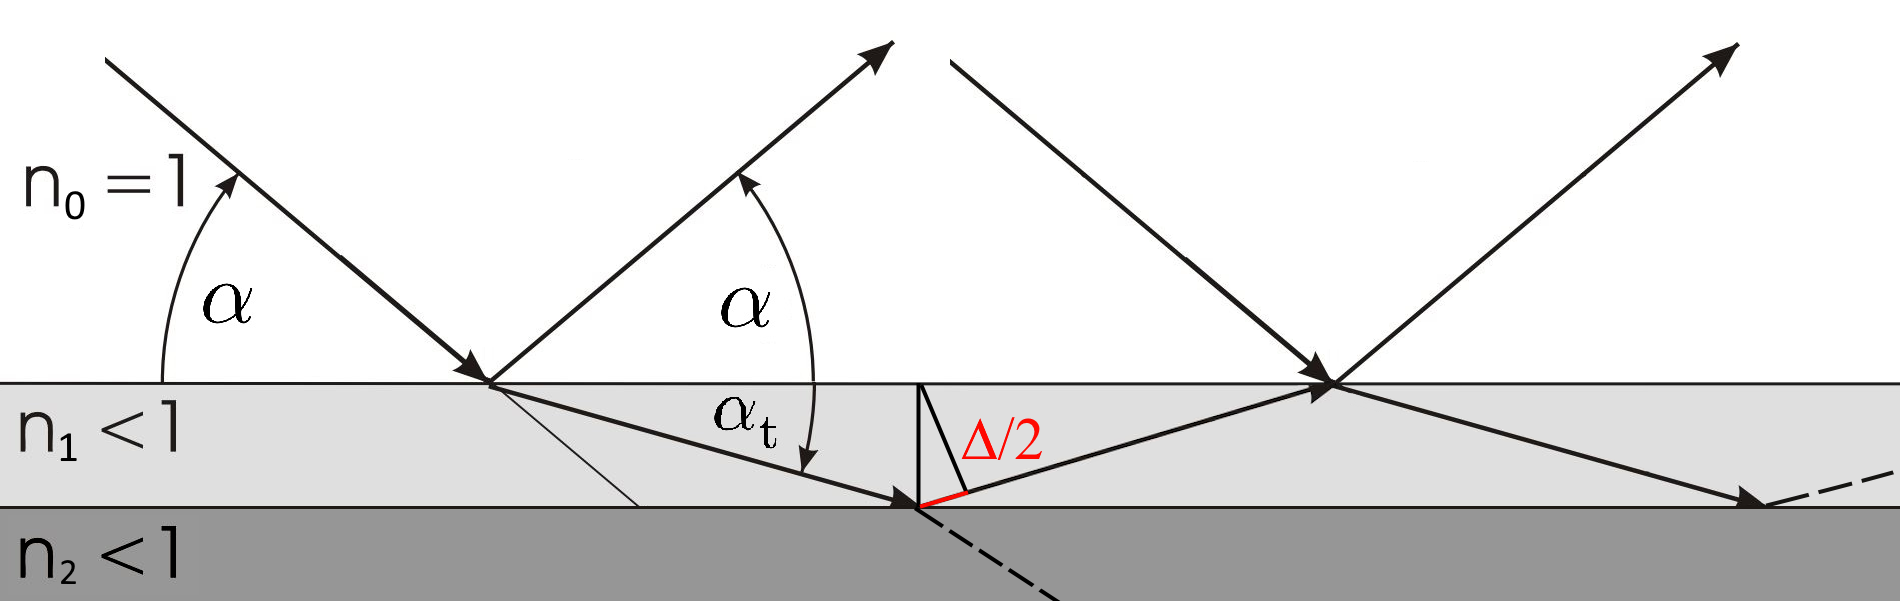
\includegraphics[scale=0.3]{Ressourcen/schicht.png}
  \caption{Querschnitt des Modells einer dünnen Schicht auf einem Substrat,\\ welches an der Grenzfläche ebenfalls reflektiv ist. Der halbe Gangunterschied \\ ist rot hervorgehoben.}\label{fig:3}
\end{figure}
Konstruktive Interferenz kann in diesem Fall auftreten, falls der effektive Gangunterschied des eingedrungenen Strahls ein mehrfaches der Wellenlänge der betrachteten Strahlung ist.
Je nachdem, wie oft der Strahl in der dünnen Schicht zwischen der Grenze von Vakuum und Substrat hin und herläuft, modifiziert sich seine resultierende Intensität mit den verschiedenen Reflexions- und Transmissionskoeffizienten $r$,$t$ der Grenzübergänge.
Durch Nutzung von Relationen welche aus den Fresnelschen Formeln folgen, ergibt sich die Formel
\begin{align}
  r_\text{ges}= \frac{r_{0\to1}+r_{1\to2}p^2}{1+r_{0\to1}r_{1\to2}p^2}\text{.}\label{eqn:schicht}
\end{align}
Die Indizes der Reflexionskoeffizienten geben an, zwischen welchen unterschiedlichen Medien der Übergang stattfindet und im Faktor $p^2=e^{ik\Delta_\text{eff}}\approx e^{ik_\text{z,0}d} \approx e^{2ik}$ mit dem transmittierten Wellenvektor senkrecht zur Grenzfläche $k_\text{z,0}$ und der Schichtdicke $d$ wird der Gangunterschied der Wellenbündel berücksichtigt.
Wie bereits aus der Formel ersichtlich, treten für die Reflexivität $R_\text{ges}=|r_\text{ges}|^2$ Oszillationen auf.
Diese werden Kiessig-Oszillationen genannt und weisen die Periode, den Abstand zwischen zwei Maxima 
\begin{align}
  T_\alpha = \frac{\lambda}{2d}
\end{align}
auf, worüber die Schichtdicke indirekt bestimmt werden kann\cite{kiessig}.
\subsection{Reflexion und Transmission an Mehrschichtsystemen}\label{subsec:multilevel}
Die oben genannten physikalischen Prozesse bei Brechung von Röntgenstrahlung an einer Schicht treten, wenn auch weitaus schwierieger zu charakterisieren, ebenfalls bei Mehrschichtigen System wie etwa in \autoref{fig:4} abgebildet auf.
An jeder Grenzfläche wird der Lichtstrahl sowohl gebrochen und transmittiert als auch reflektiert, beschrieben durch die Intensitätskoeffizienten $R_\text{j}$ und $T_\text{j}$, wobei $\text{j}$ der Index des jeweiligen Grenzübergangs ist.
Ausgehend von $R_\text{n+1}$, der Annahmem, dass ins Substrat eingedrungene Licht aufgrund von vollständiger Absorption nicht wieder am Boden reflektiert wird, können die Transmissions- und Reflexionskoeffizienten rekursiv mittels des Parratt-Algorithmus berechnet werden.
Dies erfolgt mittels der Gleichung
\begin{align}
  X_\text{j} = e^{-2ik_\text{z,j}z_\text{j}}\frac{r_\text{j,j+1}+X_\text{j+1}e^{2ik_\text{z,j+1}z_\text{j}}}{1+r_\text{j,j+1}X_\text{j+1}e^{2ik_\text{z,j+1}z_\text{j}}}
\end{align}
inklusive der Reflexionskoeffizienten
\begin{align}
  r_\text{j,j+1}=\frac{k_\text{z,j}-k_\text{z,j+1}}{k_\text{z,j}+k_\text{z,j+1}}
\end{align}
und den Wellenvektorkomponenten
\begin{align}
  k_\text{z,j}&=\frac{2\pi}{\lambda}\sin{\alpha}\\
  k_\text{z,j+1}&=\frac{2\pi}{\lambda}\sqrt{n^2-cos^2{\alpha}}\text{.}
\end{align}
\begin{figure}[H]
  \centering
  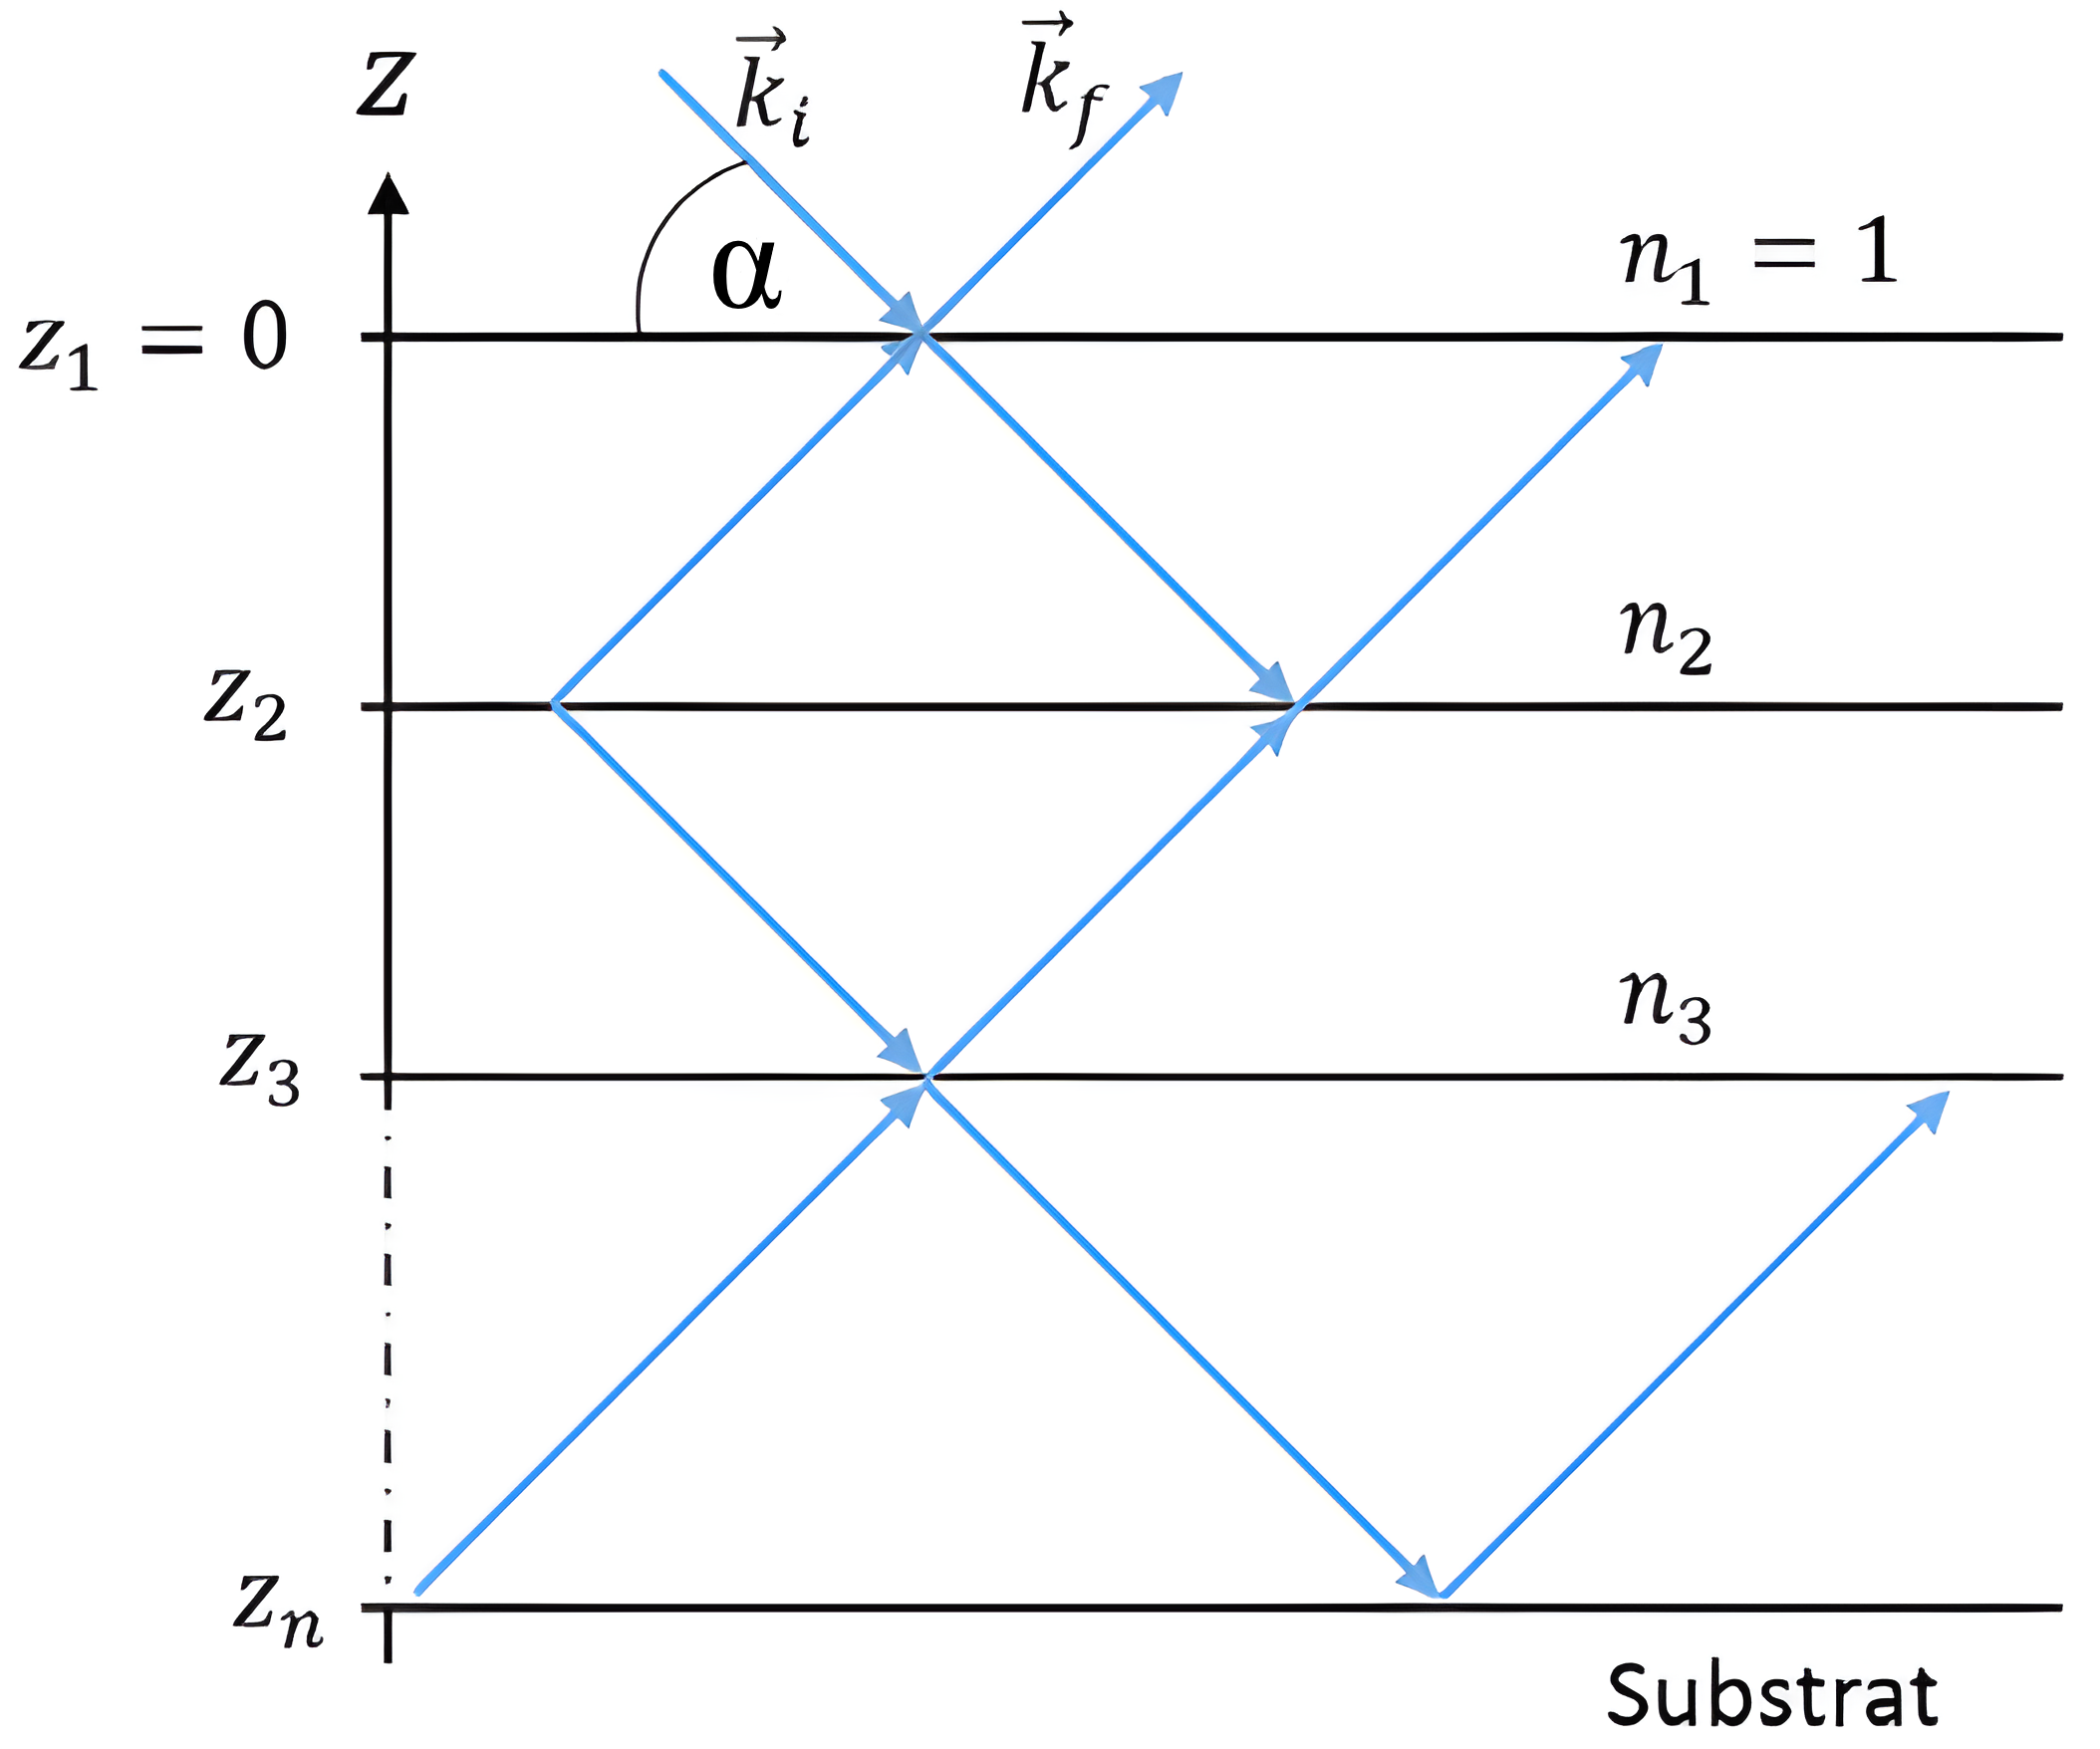
\includegraphics[scale=0.12]{Ressourcen/mehrschicht.png}
  \caption{Skizzierung eines n-schichtigen Systems, mit n individuellen\\ Grenzflächen und Brechungsindizes\cite{juwi2015}}\label{fig:4}
\end{figure}
\subsection{Rauigkeit}{\label{subsec:rauigkeit}}
Um die unebenheit der untersuchten Probe zu berücksichtigen, müssen einige Korrekturen eingeführt werden.
Mit der Annahme, dass die mittlere Abweichung von der durchschnittlichen Schichthöhe $\sigma$ weitaus kleiner als die Schichtdicke ist, kann die Unebenheit der Oberfläche annähernd Gaußverteilt beschrieben werden.
Der transformierte Reflexionskoeffizient
\begin{align}
    r_\text{j,j+1}'=r_\text{j,j+1}\cdot e^{-2k_\text{z,j}k_\text{z,j+1}\sigma^2}
\end{align}
reicht im gegebenen Kontext als Approximation aus.
\subsection{Geometriefaktor}
Der Geometriefaktor $ G $ spielt eine Rolle bei der Berücksichtigung des Einfallswinkels, ab dem der gesamte Strahl die Probenoberfläche erreicht und reflektiert wird. Dieser kritische Einfallswinkel wird als Geometriewinkel $ \alpha_g $ bezeichnet. Wenn der Einfallswinkel $ \alpha_i $ kleiner als der Geometriewinkel ist, wird der Geometriefaktor $ G $ durch die folgende Beziehung definiert:
\begin{align}
G = \frac{D \sin(\alpha_i)}{d_0}\label{eqn:G}
\end{align}
Hierbei ist $ D $ der Durchmesser der Probenoberfläche und $ d_0 $ die Höhe des Strahls. Wenn $ \alpha_i $ größer als $ \alpha_g $ ist, wird $ G $ als 1 angenommen.
Wenn $ \alpha_i $ sehr klein ist, überstreicht der Strahl eine größere Fläche als die Probenoberfläche, sodass nicht die gesamte eingestrahlte Intensität von der Probenoberfläche reflektiert wird, die in den Detektor gelangen kann. Dies führt zu einem Rückgang der Reflektivität im Bereich sehr kleiner Winkel $ \alpha_i < \alpha_g $. Der Geometriefaktor $ G $ berücksichtigt diesen Effekt und wird als Verhältnis der Strahlbreite $ D \sin(\alpha_i) $, die die Probenoberfläche erreicht, zur Gesamtstrahlbreite $ d_0 $ definiert.
\section{Aufbau}
Das Diffraktometer besteht aus drei Komponenten: der Röntgenquelle (links), dem Probentisch (mittig) und dem Detektor (rechts).
\begin{figure}[H]
  \centering
  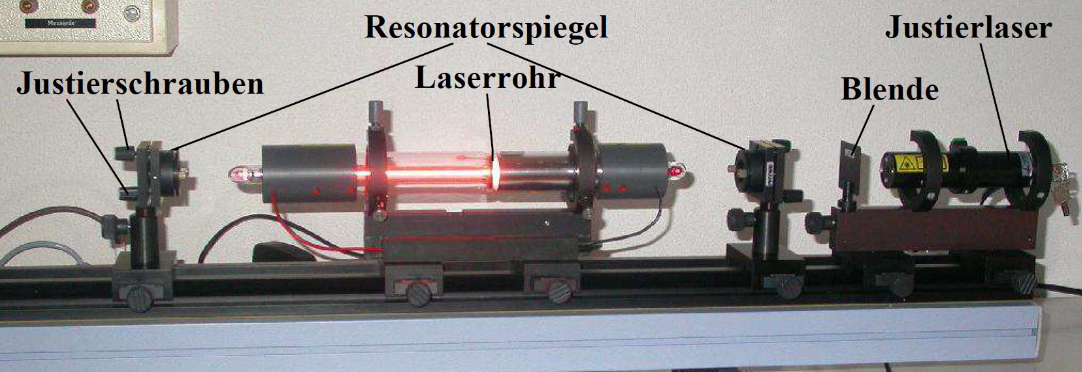
\includegraphics[scale=0.12]{Ressourcen/aufbau.png}
  \caption{Beschrifteter Versuchsaufbau}\label{fig:5}
\end{figure}
\subsection{Röntgenquelle}
In der Röntgenquelle wird ein Elektronenstrahl von 35 mA mit einer Spannung von 40 kV auf eine schräge Kupferanode beschleunigt. Im Kupfer verlieren die Elektronen ihre kinetische Energie durch zufällige Stöße in beliebigen Portionen, was zum kontinuierlichen Spektrum der Bremsstrahlung führt (beschleunigte Ladungen emittieren Photonen). Zusätzlich entstehen materialspezifische Peaks spezieller Energien, die charakteristische Röntgenstrahlung, die durch Ionisation der Kupferatome aus bestimmten Energieniveaus heraus entsteht, wenn die Elektronen von höheren Niveaus nachrutschen. Die charakteristische Röntgenstrahlung $K_{\alpha_1}$ von 8,905 keV wird für diesen Versuch verwendet.
Die in der Röntgenröhre erzeugte Röntgenstrahlung wird durch Blenden im Raumwinkel eingeschränkt und dann über einen Göbelspiegel frequenz- und winkelabhängig in die gewünschte Richtung parallelisiert. Durch eine weitere Blendenanordnung wird der Strahl weiter eingeschränkt. Der Göbelspiegel besteht aus mehreren dünnen Schichten mit abwechselnden Brechungsindizes, deren Dicke so gewählt wird, dass es für die gewünschte Frequenz nach dem Prinzip der Braggreflexion zu konstruktiver Interferenz kommt. Die parabolische Geometrie unterstützt die Parallelisierung des Strahls. Die in diesem Versuch diskutierten Kiessig-Oszillationen an dünnen Schichten treten auch hier auf, spielen jedoch im Vergleich zur Braggreflexion eine untergeordnete Rolle.
\subsection{Probentisch}
Der Probentisch kann mittels Elektromotoren so eingestellt werden, dass die Probe optimal in der Drehachse von Röntgenstrahl und Detektor liegt, wobei dieselbe Stelle der Probe möglichst mittig im Strahl bleibt. Auf dem Probentisch liegt ein quadratisches Stück eines mit einem dünnen Polymerfilm beschichteten Siliziumwafers.
\subsection{Detektor}
Der Detektor ermittelt über die Ionisierungswirkung von Röntgenstrahlen die Intensität des einfallenden Röntgenstrahls.
In diesem Versuch wird die, ausgehend vom Glanzwinkel (größter Winkel mit Totalreflexion), mit steigendem Winkel abnehmende Intensität des reflektierten Strahls gemessen. Hierbei zeigen sich periodische, positive Abweichungen vom grundsätzlich exponentiellen Abfall. Diese Abweichungen sind die sogenannten Kiessig-Oszillationen, die Rückschlüsse auf Rauigkeit und Schichtdicke liefern.
\section{Durchführung}\label{sec:durchfuehrung}
\subsection{Justierung des Diffraktometers}
\subsubsection{Detektorscan}
Mit einem sogenannten Detektorscan wird ohne Probe der Röntgenstrahl vermessen. Die hierbei ermittelte Intensitätsverteilung entspricht grob einer Gaußkurve, deren Maximum die Mitte des Strahls definiert. Bei uns zeigte sich auf der linken Flanke ein Buckel, der sich durch eine Änderung der Blendenapparatur an der Röntgenquelle deutlich verkleinern ließ. Die Auswertung der gefitteten Gaußkurve und entsprechende Justierung des Diffraktometers erfolgt innerhalb der Software ohne menschliche Interpretation.
\subsubsection{X-Scan}
Die Probe wird zunächst in ausreichender Höhe durch einen X-Scan in X-Richtung (Vor und Zurück) durch den Strahl bewegt. Dabei zeigt sich ein Bereich mit Abschattung. In diesem Bereich kann die Probe frei positioniert werden.
\subsubsection{Z-Scan}
Über einen Z-Scan wird die Probe in Z-Richtung (Auf und Ab) in und durch den Röntgenstrahl bewegt. Dabei verbleibt die gemessene Intensität zunächst unverändert auf dem Niveau des Detektorscans. Sobald die Probe einen Teil des Röntgenstrahls abschattet, sinkt die Intensität rapide ab, bis der Strahl komplett abgeschirmt wird und der Detektor nur noch Streustrahlung aufzeichnet. Per Augenmaß wird die halbe Abschattung markiert und als erste Näherung der idealen Z-Position gesetzt.
\subsubsection{Rockingscan}
Falls die Probe im Strahl geneigt ist, erfolgt ein Teil der Abschattung beim Z-Scan nicht durch die Seitenfläche der Probe, sondern durch die geneigte Oberfläche. Deshalb erfolgt ein sogenannter Rockingscan. Hierbei werden Röntgenquelle und Detektor so gedreht, als würde die Probe gedreht. Der Detektor zeichnet dabei ein Signal auf, das einem Dreieck ähnelt. Ist das Dreieck nicht symmetrisch, so muss die Y-Position nachgestellt werden, bis der Strahl die Probe immer in der Mitte trifft. Liegt die Spitze des Dreiecks nicht auf der Nullposition, so ist die Probe verkippt und die Nullgrad-Position muss angepasst werden. Entsprechende Korrekturwerte müssen ausprobiert werden.
Da die Korrektur der Verkippung die Probe beim Z-Scan parallel ausrichtet, verschwindet die dadurch verursachte Abweichung von der mittleren Höhe. Es folgt eine weitere Runde Z-Scan und Rockingscan, diesmal mit größerer Genauigkeit.
\subsection{Messvorgang des Polymerfilms}
Der Messvorgang beginnt mit einem Reflektivitätsscan, bei dem der Einfallswinkel $\alpha_i$ und der Detektorwinkel $\alpha_f$ gleich sind. Der Scanbereich reicht von 0° bis 2,5°, mit Schrittweiten von 0,005° und einer Messzeit von mindestens 5 Sekunden pro Messpunkt.
Ein „Diffuser Scan“ wird durchgeführt, um den Anteil der gestreuten Intensität zu bestimmen, wobei der Detektorwinkel um 0,1° gegenüber dem Einfallswinkel verschoben wird. Die Messergebnisse werden im .raw-Format gespeichert, mit dem Programm „File Exchange“ in .uxd umgewandelt und auf einem USB-Stick gesichert.

\section{Auswertung}\label{sec:auswertung}
\subsection{Fehler und Messunsicherheiten}\label{subsec:fehler-und-messunsicherheiten}
Jegliche Fehlerfortpflanzungen und Berechnungen mit Messunsicherheiten finden durch das Python-Package Uncertainties\cite{uncertainties} statt.
Somit werden einmal alle bekannten Variablen einmal mit einer speziellen Funktion aus Uncertainties festgelegt.
Bei allen nachfolgenden Berechnungen erfolgen die benötigten Fortpflanzungen durch Uncertainties automatisch.
Die Formel für die Fehlerfortpflanzung ist
\begin{align}
  \Delta y=\sum_{i=1}^n\left|\frac{\delta f\left(x_1, \ldots, x_n\right)}{\delta x_i}\right| \Delta x_i.\text{.}\label{gauss}
\end{align}
und die Formel für den Mittelwert/ das arithmetische Mittel ist
\begin{align}
  \bar{x}=\frac{1}{n}\sum_{i=1}^n x_i\label{mittel}
\end{align}
Wie die Ableitungen bestimmt werden ist in der \href{https://readthedocs.org/projects/uncertainties-python-package/downloads/pdf/latest/}{Technischen Dokumentation} selbst nachzulesen.
\subsection{Bestimmung der Halbwertsbreite und der maximalen Intensität}
Zur Analyse des Detektorscans wurde eine Gaußfunktion der Form
\begin{align*}
I(\theta) = I_{\text{max}} \exp \left( -\frac{(\theta - \theta_0)^2}{2\sigma^2} \right),
\end{align*}
an die experimentellen Daten angepasst wie in \autoref{fig:6} zu sehen ist,wobei $I(\theta)$ die Intensität bei der Position $\theta$, $I_{\text{max}}$ die maximale Intensität, \(\theta_0\) die Position des Intensitätsmaximums und \(\sigma\) die Standardabweichung der Gaußverteilung ist.
\begin{figure}[H]
  \centering
  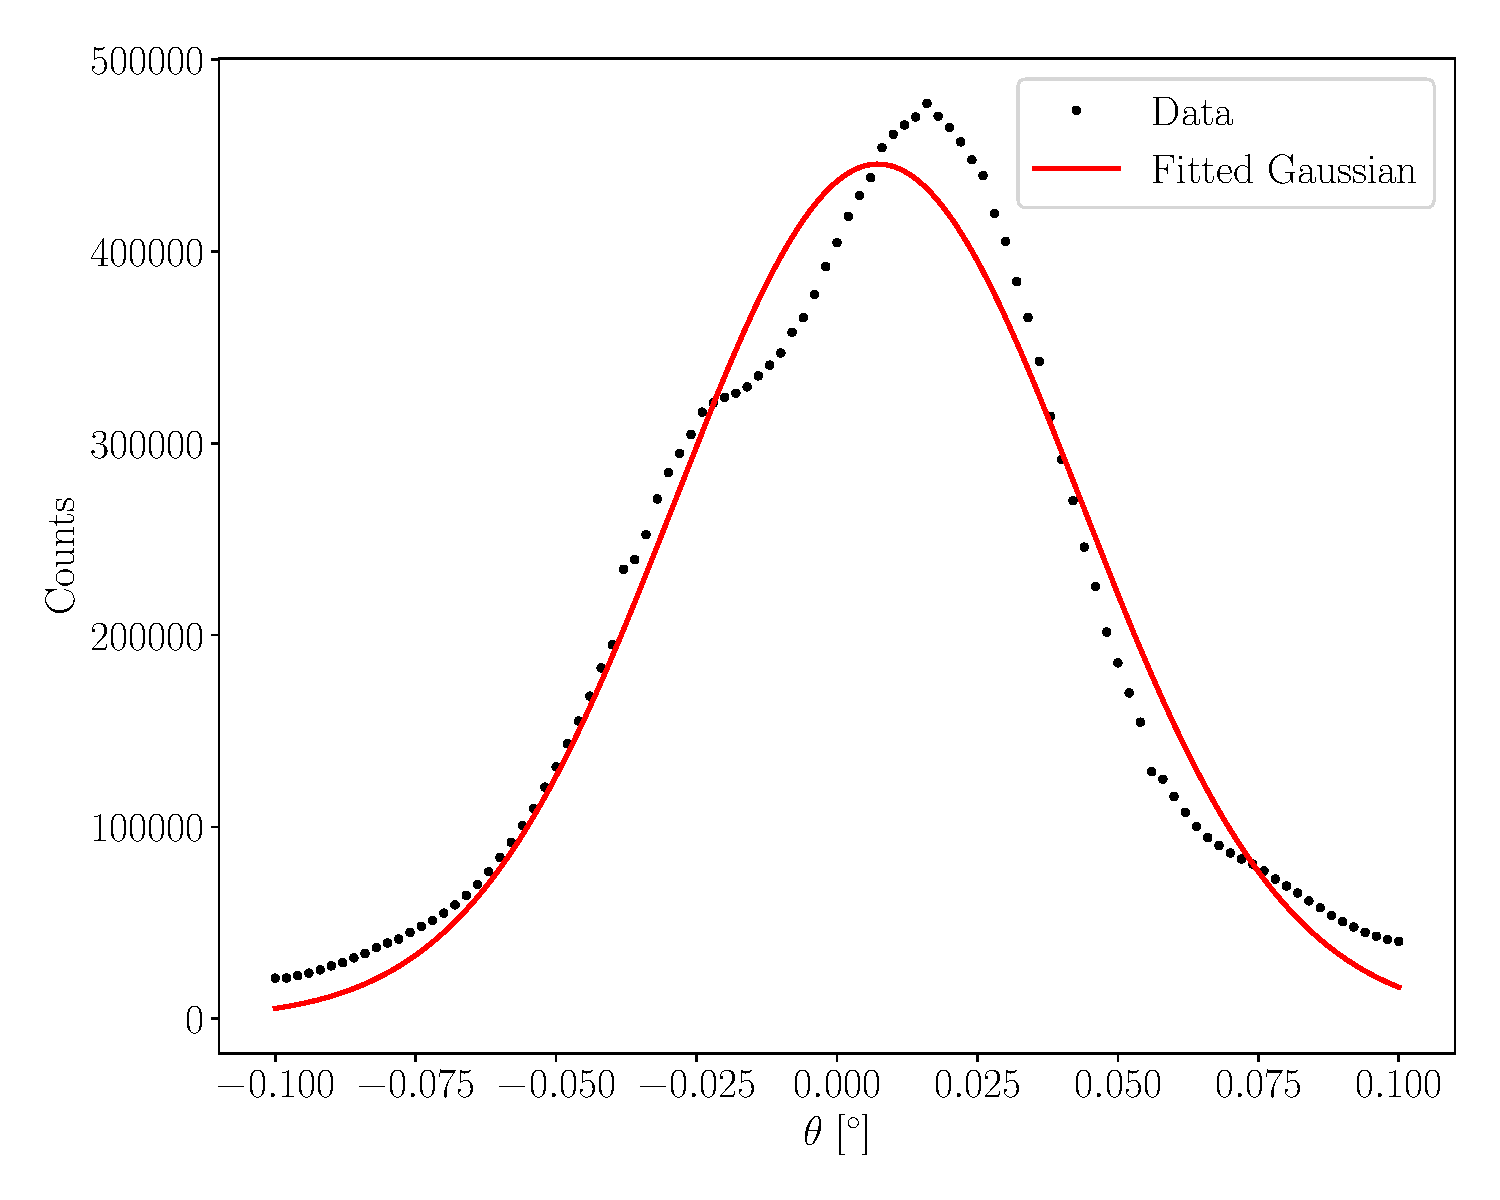
\includegraphics[scale=0.5]{Ressourcen/detektor1.pdf}
  \caption{Messdaten sowie zugehöriger Gaussfit.}\label{fig:6}
\end{figure}
\begin{enumerate}
    \item Zunächst wurden die experimentellen Intensitätsdaten gegen die Position \(\theta\) geplottet.
    \item Anschließend wurde die Gaußfunktion mittels der SciPy Funktion $\text{curve\_fit}$ an die Daten angepasst\cite{scipy}. Dies wurde mit Hilfe der Methode der kleinsten Quadrate durchgeführt, um die Parameter \(I_{\text{max}}\), \(\alpha_0\) und \(\sigma\) zu bestimmen.
    \item Die maximale Intensität \(I_{\text{max}}\) wurde direkt aus der Anpassung erhalten.
    \item Die Halbwertsbreite (Full Width at Half Maximum, FWHM) der Gaußfunktion wurde durch die Beziehung zwischen der Halbwertsbreite und der Standardabweichung \(\sigma\) berechnet. Für eine Gaußfunktion gilt:
    \begin{align*}
    \text{FWHM} = 2 \sqrt{2 \ln 2} \, \sigma \approx 2.355 \, \sigma.
    \end{align*}
\end{enumerate}
Infolge des beschriebenen Verfahrens ergibt sich die Maximale Intensität 
\begin{align*}
  I_{\text{max}} = 445506\text{ Counts},
\end{align*}
sowie die Halbwertsbreite
\begin{align*}
  \text{FWHM} = \SI{0.086(0.002)}{\degree}\text{.}
\end{align*}
\subsection{Probenscan und Ideale Fresnelreflektivität}
Nach Datenaufnahme des Proben- sowie Diffusen Scans gemäß \autoref{sec:durchfuehrung} kann die Hintergrundintensität bereinigt werden, indem die Scans voneinander abgezogen werden.
Durch Bestimmung der Strahlbreite $d_0$ und der Probenlänge $D$ mittels \hyperref[sec:durchfuehrung]{X- und Z-Scan} kann der Geometriefaktor $G$
und der Geometriewinkel
\begin{align*}
  \alpha_\text{g, berechnet}=\arcsin\left(\frac{d_0}{D}\right) \cdot \frac{360}{2 \pi}=\SI{0.458(0.062)}{\degree}
\end{align*}
entsprechend \autoref{eqn:G} berechnet werden.
Ebenso können die kritischen Winkel von Silizium und Polysterol $\alpha_\text{c,Si}, \alpha_\text{c,Po}$ entsprechend \autoref{eqn:a_krit} und den theoretischen Dispersionen $\delta$, welche der Anleitung entnommen wurden, zu
\begin{align*}
  \alpha_\text{c,Si}&=\SI{0.223}{\degree}\\
  \alpha_\text{c,Po}&=\SI{0.151}{\degree}
\end{align*}
berechnet werden.
Sind diese Komponenten alle bekannt, können die gemessene Intensität, die hintergrundbereinigte Intensität, die geometrisch korrigierte Intensität und die Ideale Fresnelintensität entsprechend \autoref{eqn:fresnel} grafisch Dargestellt werden.
Dies ist in \autoref{fig:7} zu sehen.
\begin{figure}[H]
  \centering
  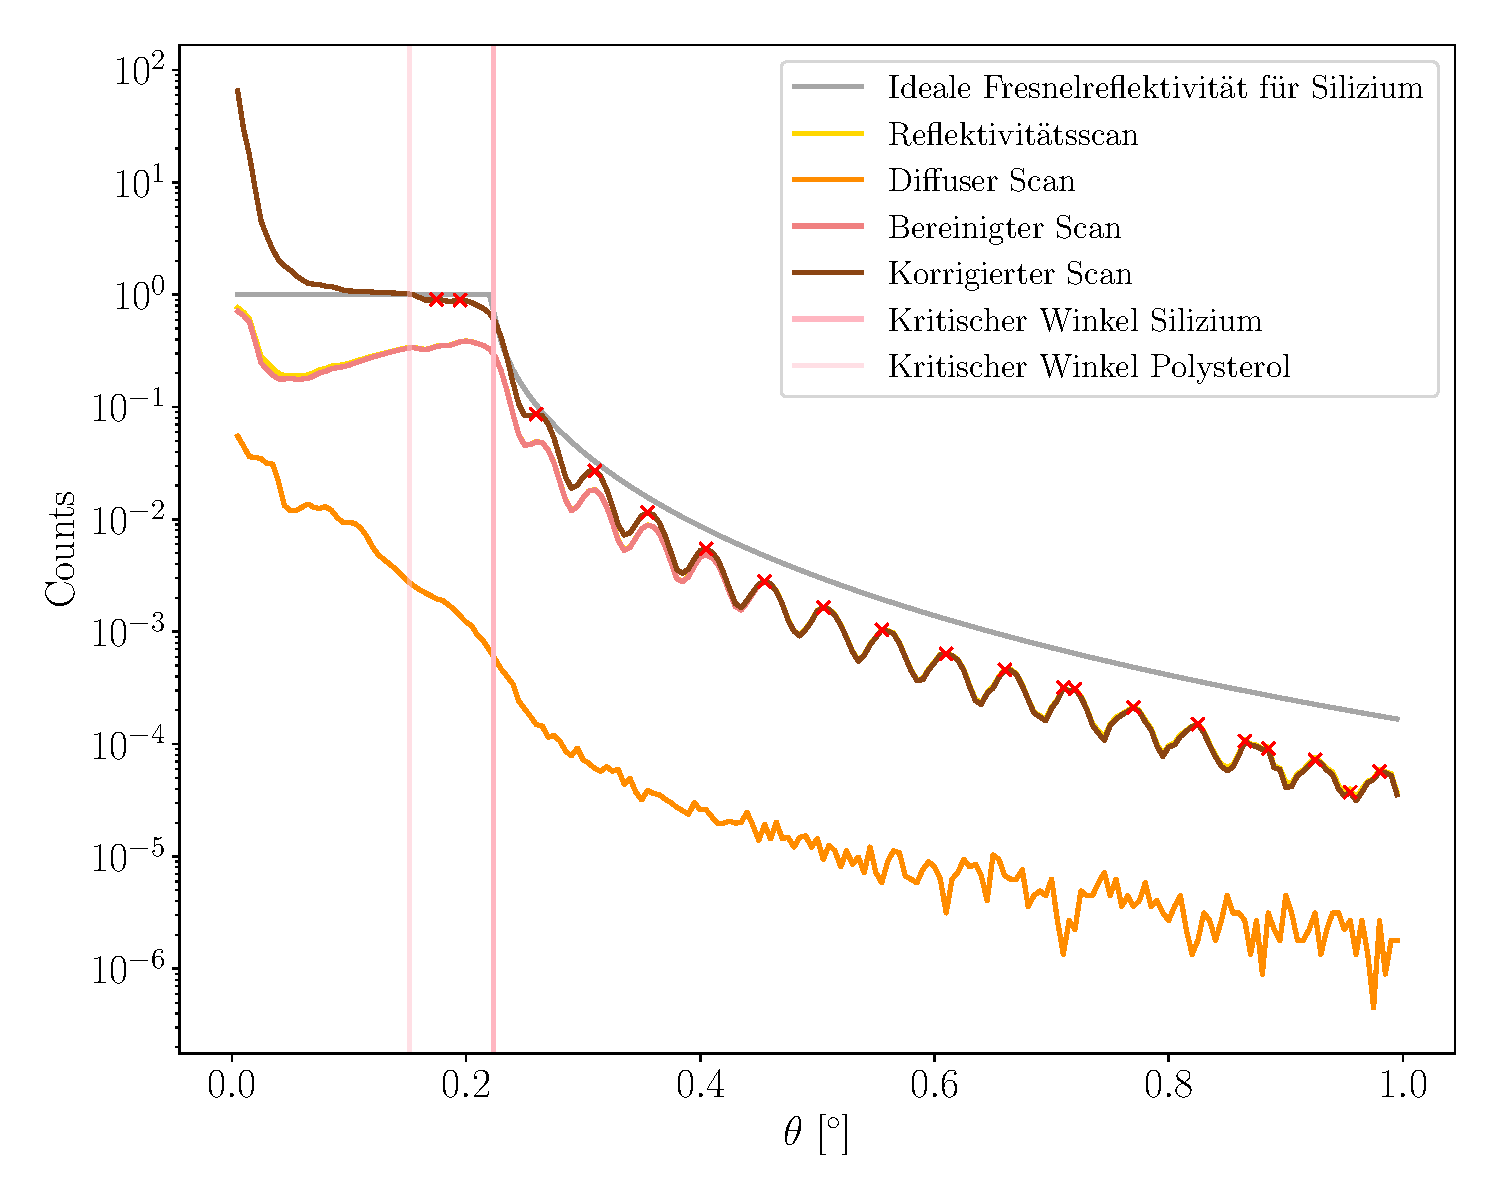
\includegraphics[scale=0.6]{Ressourcen/probe.pdf}
  \caption{Alle oben genannten Intensitäten, inklusive der Kritischen Winkel für Silizium und Polysterol und der Intensitätspeaks.}\label{fig:7}
\end{figure}
\subsection{Vergleich des Geometriewinkels}
Mithilfe eines linearen Fits an die Relevanten Daten nach dem gemessenen Intensitätsmaximum wie in \autoref{fig:8} dargestellt des Probenscans kann der entsprechende Winkel der Intensität $I=0$ als
\begin{align*}
  \alpha_\text{g,gemessen}=\SI{0.389(0.011)}{\degree}
\end{align*}
bestimmt werden. 
\begin{figure}[H]
  \centering
  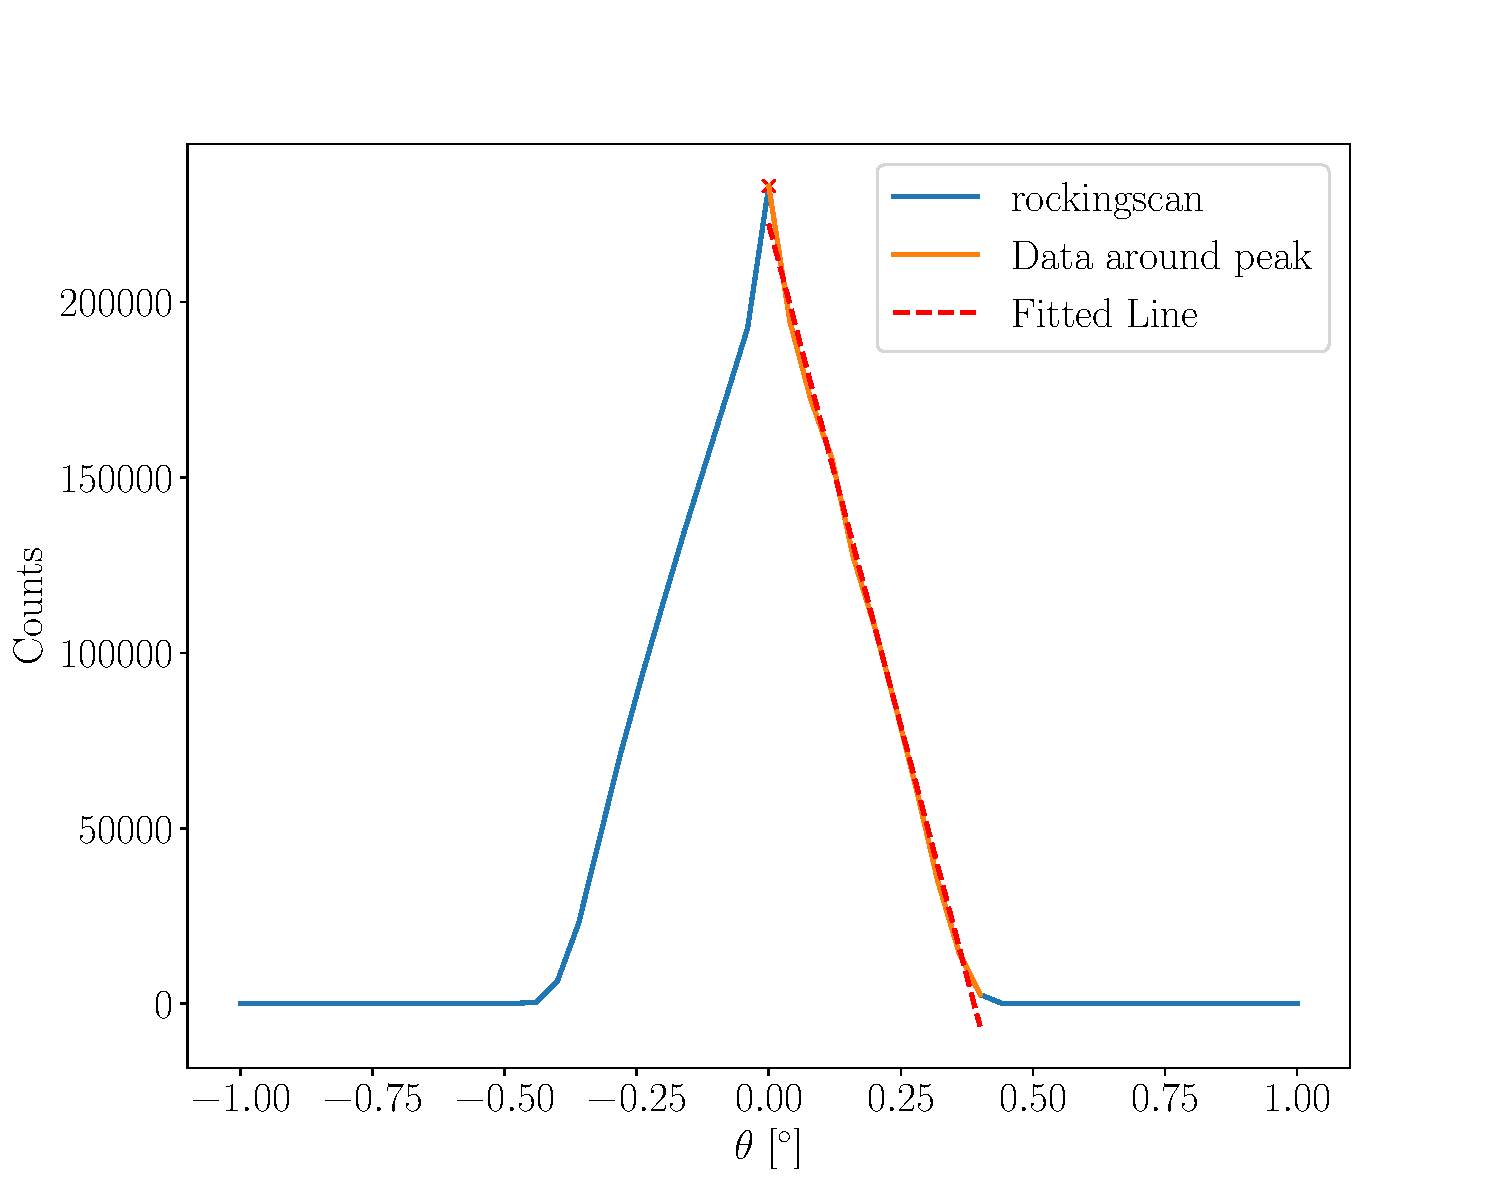
\includegraphics[scale=0.6]{Ressourcen/rocking.pdf}
  \caption{Messdaten und Ausgleichsgerade des Rockingscans.}\label{fig:8}
\end{figure}
\subsection{Abschätzung der Schichtdicke}
Wie in \autoref{subsec:interferenz} beschrieben kann die Schichtdicke zunächst aus den Abständen der Reflexivitätsmaxima abgeschätzt werden.
Unter Nutzung der in \autoref{fig:7} gekennzeichneten Maxima folgt eine erste Schätzung der Schichtdicke als
\begin{align*}
  d_\text{0} = \SI{1.7(0.5)e-09}{\meter}\text{.}
\end{align*}

\section{Diskussion}\label{sec:diskussion}

\section{Literaturverzeichnis}\label{sec:literaturverzeichnis}
\printbibliography[heading = none]
\newpage

\section{Anhang}\label{sec:anhang}

\end{document}
